
%(BEGIN_QUESTION)
% Copyright 2007, Tony R. Kuphaldt, released under the Creative Commons Attribution License (v 1.0)
% This means you may do almost anything with this work of mine, so long as you give me proper credit

Calculate an appropriate control valve size ($C_v$ and nominal pipe size) for this water flow control application, assuming a maximum flow rate of 300 GPM:

$$\includegraphics[width=15.5cm]{i01823x01.eps}$$

Assume a vertical distance of 195 feet from the pump discharge to the average water level in the storage tank.

\vfil

\underbar{file i01823}
\eject
%(END_QUESTION)





%(BEGIN_ANSWER)

This is a graded question -- no answers or hints given!

%(END_ANSWER)





%(BEGIN_NOTES)

Recall that the purpose of a {\it pump curve} is to predict the discharge pressure of a pump at full shaft speed given a certain amount of liquid flow through it.  We may use the pump curve in this case to tell the pump's discharge pressure will be 105 PSI at a flow rate of 300 GPM.  This will be the control valve's upstream pressure.

In order to determine the differential pressure across the valve -- which we will need in order to calculate its necessary $C_v$ -- we must determine the valve's downstream pressure.  In this particular process, downstream pressure is simply the hydrostatic ``head'' of the water tower's 195 foot height.  A column of water 195 feet high generates a hydrostatic pressure of approximately 84.54 PSI.  This means the control valve's differential pressure will be 105 PSI $-$ 84.54 PSI = 20.46 PSI.

\vskip 10pt

Control valve $\Delta P$ = 20.46 PSID

$$Q = C_v \sqrt{\Delta P \over G_f}$$

$C_v$ = 66.32

\vskip 10pt

This will require a nominal pipe size of 2 inches, assuming a $C_d$ of 25 for a characterized ball valve (actual $d$ calculated value = 1.629 inches).

%INDEX% Final Control Elements, valve: sizing
%INDEX% Process: water storage tank (elevated)

%(END_NOTES)


